%%
%%
%% The first command in your LaTeX source must be the \documentclass command.
\documentclass[sigchi, 12pt, nonacm=true, timestamp=true, screen=true]{acmart}

%%
%% \BibTeX command to typeset BibTeX logo in the docs
\AtBeginDocument{%
  \providecommand\BibTeX{{%
    \normalfont B\kern-0.5em{\scshape i\kern-0.25em b}\kern-0.8em\TeX}}}

%% Rights management information.  This information is sent to you
%% when you complete the rights form.  These commands have SAMPLE
%% values in them; it is your responsibility as an author to replace
%% the commands and values with those provided to you when you
%% complete the rights form.
%%\setcopyright{acmcopyright}
%%\copyrightyear{2018}
%%\acmYear{2018}
%%\acmDOI{10.1145/1122445.1122456}

%% These commands are for a PROCEEDINGS abstract or paper.
%%\acmConference[Woodstock '18]{Woodstock '18: ACM Symposium on Neural
%%  Gaze Detection}{June 03--05, 2018}{Woodstock, NY}
%%\acmBooktitle{Woodstock '18: ACM Symposium on Neural Gaze Detection,
%%  June 03--05, 2018, Woodstock, NY}
%%\acmPrice{15.00}
%%\acmISBN{978-1-4503-9999-9/18/06}


%%
%% Submission ID.
%% Use this when submitting an article to a sponsored event. You'll
%% receive a unique submission ID from the organizers
%% of the event, and this ID should be used as the parameter to this command.
%%\acmSubmissionID{123-A56-BU3}

%%
%% The majority of ACM publications use numbered citations and
%% references.  The command \citestyle{authoryear} switches to the
%% "author year" style.
%%
%% If you are preparing content for an event
%% sponsored by ACM SIGGRAPH, you must use the "author year" style of
%% citations and references.
%% Uncommenting
%% the next command will enable that style.
%%\citestyle{acmauthoryear}

\setcopyright{none}

\usepackage{hyperref}
\usepackage{subfiles}
\usepackage{url}
\usepackage{soul}

%%\citestyle{acmauthoryear}

%%
%% end of the preamble, start of the body of the document source.
\begin{document}

%%
%% The "title" command has an optional parameter,
%% allowing the author to define a "short title" to be used in page headers.
\title{Team 5 Project Proposal - MovieEdge}

%%
%% The "author" command and its associated commands are used to define
%% the authors and their affiliations.
%% Of note is the shared affiliation of the first two authors, and the
%% "authornote" and "authornotemark" commands
%% used to denote shared contribution to the research.

\author{Rocko Graziano}
\email{rpgraziano@gatech.edu}
\affiliation{%
  \institution{Georgia Tech OMSCS}
}
\author{Daniel Klass}
\email{dklass3@gatech.edu}
\affiliation{%
	\institution{Georgia Tech OMSCS}
}
\author{Yi Sun}
\email{ysun428@gatech.edu}
\affiliation{%
	\institution{Georgia Tech OMSCS}
}
\author{Jonathan Tay}
\email{jtay6@gatech.edu}
\affiliation{%
	\institution{Georgia Tech OMSCS}
}


%%
%% By default, the full list of authors will be used in the page
%% headers. Often, this list is too long, and will overlap
%% other information printed in the page headers. This command allows
%% the author to define a more concise list
%% of authors' names for this purpose.
%\renewcommand{\shortauthors}{Trovato and Tobin, et al.}

%%
%% The abstract is a short summary of the work to be presented in the
%% article.
\begin{abstract}
	We present \textbf{MovieEdge}, a recommendation system which provides an interactive visualization interface for users.
\end{abstract}
%%
%% The code below is generated by the tool at http://dl.acm.org/ccs.cfm.
%% Please copy and paste the code instead of the example below.
%%
%%\begin{CCSXML}
%%<ccs2012>
%% <concept>
%%  <concept_id>10010520.10010553.10010562</concept_id>
%%  <concept_desc>Computer systems organization~Embedded systems</concept_desc>
%%  <concept_significance>500</concept_significance>
%% </concept>
%% <concept>
%%  <concept_id>10010520.10010575.10010755</concept_id>
%%  <concept_desc>Computer systems organization~Redundancy</concept_desc>
%%  <concept_significance>300</concept_significance>
%% </concept>
%% <concept>
%%  <concept_id>10010520.10010553.10010554</concept_id>
%%  <concept_desc>Computer systems organization~Robotics</concept_desc>
%%  <concept_significance>100</concept_significance>
%% </concept>
%% <concept>
%%  <concept_id>10003033.10003083.10003095</concept_id>
%%  <concept_desc>Networks~Network reliability</concept_desc>
%%  <concept_significance>100</concept_significance>
%% </concept>
%%</ccs2012>
%%\end{CCSXML}

%%\ccsdesc[500]{Computer systems organization~Embedded systems}
%%\ccsdesc[300]{Computer systems organization~Redundancy}
%%\ccsdesc{Computer systems organization~Robotics}
%%\ccsdesc[100]{Networks~Network reliability}

%%
%% Keywords. The author(s) should pick words that accurately describe
%% the work being presented. Separate the keywords with commas.
%%\keywords{movies, DVA, lorem ipso}

%% A "teaser" image appears between the author and affiliation
%% information and the body of the document, and typically spans the
%% page.
%%\begin{teaserfigure}
%%  \includegraphics[width=\textwidth]{sampleteaser}
%%  \caption{Seattle Mariners at Spring Training, 2010.}
%%  \Description{Enjoying the baseball game from the third-base
%%  seats. Ichiro Suzuki preparing to bat.}
%%  \label{fig:teaser}
%%\end{teaserfigure}

%%
%% This command processes the author and affiliation and title
%% information and builds the first part of the formatted document.
\maketitle
\section{Introduction}
\subfile{sections/introductionV2}
\section{Related Work}
\subfile{sections/relatedwork}
\section{Heilmeier Quesitons}
\subfile{sections/heilmeier}

%\section{Project Overview}
%\subfile{sections/today}
%\subfile{sections/novelty}
%\subfile{sections/audience}
%\subfile{sections/difference-impact}
%
%\section{Project Details}
%\subfile{sections/risks-payoff}
%\subfile{sections/costs}	
%\subfile{sections/projectplan}
%\section{Conclusion}
%\subfile{sections/conclusion}

%% the bibliography file.


%\bibliographystyle{apalike}
\bibliographystyle{ACM-Reference-Format}
\bibliography{sections/bibliography}

%
%\begin{figure*}
%	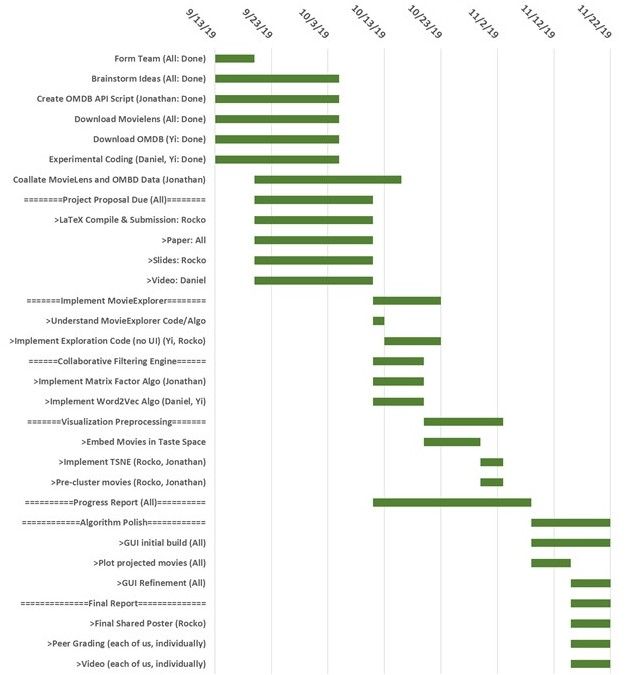
\includegraphics{ProjectPlan}
%	\caption{Project Plan}
%	\label{fig:ProjectPlan}
%\end{figure*}

\begin{figure*}
	\centering
	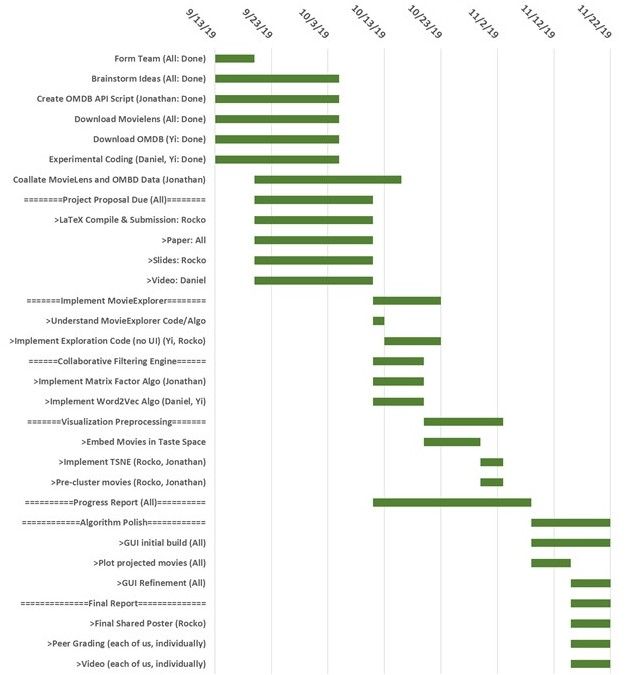
\includegraphics[width=1\linewidth]{ProjectPlan}
	\caption[Project Plan]{Plan of Activities}
	\label{fig:projectplan}
\end{figure*}


\end{document}
\endinput

%%
%% End of file `sample-sigconf.tex'.
